\documentclass[runningheads]{llncs}

% XeLaTeX được dùng để hiển thị tiếng Việt trực tiếp và ổn định.
\usepackage{fontspec}
\defaultfontfeatures{Ligatures=TeX}
\setmainfont{lmroman10-regular.otf}[
  BoldFont=lmroman10-bold.otf,
  ItalicFont=lmroman10-italic.otf,
  BoldItalicFont=lmroman10-bolditalic.otf
]
\setsansfont{lmsans10-regular.otf}[
  BoldFont=lmsans10-bold.otf,
  ItalicFont=lmsans10-oblique.otf,
  BoldItalicFont=lmsans10-boldoblique.otf
]
\setmonofont{lmmono10-regular.otf}[
  ItalicFont=lmmono10-italic.otf
]
\usepackage{graphicx}
\usepackage{booktabs}
\usepackage{array}
\usepackage{microtype}
\usepackage{xurl}
\usepackage[colorlinks=true,linkcolor=blue,citecolor=blue,urlcolor=blue]{hyperref}

\graphicspath{{figures/}}
\renewcommand{\UrlFont}{\ttfamily\small}
\newcommand{\tableref}[1]{\hyperref[#1]{Table~\ref*{#1}}}
\setcounter{secnumdepth}{3}
\raggedbottom

\begin{document}

\title{Báo cáo hệ thống LLM tư vấn dịch vụ hành chính giai đoạn cơ bản}
\titlerunning{Hệ thống LLM tư vấn dịch vụ hành chính}

\author{Bùi Xuân Hoan \and Phạm Lê Minh \and Phan Văn Tú}
\authorrunning{B.X. Hoan, P.L. Minh và P.V. Tú}

\institute{FPT University, Ho Chi Minh City, Vietnam\\
\email{bhoan2006@gmail.com, minhkek332@gmail.com, vantu12772@gmail.com}}

\maketitle

\begin{abstract}
Báo cáo trình bày quá trình xây dựng một chatbot hành chính cơ bản qua ba giai
đoạn. Giai đoạn đầu thiết lập luồng hoạt động giữa giao diện web, Core Backend,
AI Service và PostgreSQL bằng phản hồi mô phỏng. Giai đoạn hai bổ sung
Retrieval-Augmented Generation (RAG) trên dữ liệu giả lập nhằm kiểm tra truy xuất,
tạo bằng chứng và trả lời kèm nguồn. Giai đoạn ba sử dụng 10 thủ tục từ dữ liệu
công ty, được chuẩn hóa thành 49 đoạn thông tin, đồng thời thay phản hồi mô phỏng
bằng Qwen3-1.7B chạy cục bộ. Kết quả thực nghiệm cho thấy pipeline hoạt động xuyên
suốt, output và citation tuân thủ contract, lịch sử hội thoại được lưu và không có
lời gọi AI bên ngoài. Hệ thống hiện là nền tảng demo nội bộ, chưa phải sản phẩm
production và chưa bảo đảm độ đúng pháp lý cho mọi câu trả lời.

\keywords{Large Language Model \and RAG \and Qwen \and chatbot hành chính \and
grounded generation}
\end{abstract}

\section{Introduction}

Các thủ tục hành chính công thường bao gồm nhiều nhóm thông tin như thành phần hồ
sơ, thời gian giải quyết, lệ phí và cơ quan tiếp nhận. Người dân có thể gặp khó
khăn khi phải tự tìm kiếm và đối chiếu những nội dung này từ nhiều nguồn khác
nhau. Vì vậy, một hệ thống sử dụng mô hình ngôn ngữ lớn (Large Language Model --
LLM) có thể hỗ trợ người dùng tiếp cận thông tin thuận tiện hơn thông qua hình
thức hội thoại tự nhiên.

Mục tiêu dài hạn của dự án là phát triển một trợ lý có khả năng tiếp nhận câu
hỏi, xác định thủ tục liên quan, cung cấp câu trả lời dễ hiểu và dẫn nguồn để
người dùng kiểm tra lại. Hệ thống có thể hỗ trợ các nhu cầu phổ biến như tra cứu
thành phần hồ sơ, thời gian xử lý, lệ phí và nơi tiếp nhận. Tuy nhiên, nó chỉ đóng
vai trò hỗ trợ cung cấp thông tin, không thay thế cơ quan hành chính hoặc chuyên
gia pháp lý trong các trường hợp cần xác nhận chính thức.

Việc triển khai ngay một hệ thống LLM hoàn chỉnh có nhiều rủi ro. Dữ liệu ban đầu
có thể chưa đồng nhất, thiếu trường hoặc chưa được xác minh. Mô hình cũng có khả
năng tạo câu trả lời không có căn cứ nếu không được cung cấp nguồn phù hợp. Ngoài
ra, hệ thống còn phải giải quyết việc lưu hội thoại, bảo vệ dữ liệu, kết nối các
dịch vụ, giới hạn tài nguyên và đánh giá chất lượng. Nếu phát triển đồng thời tất
cả chức năng, nhóm khó xác định lỗi xuất phát từ dữ liệu, truy xuất, model hay
phần mềm tích hợp.

Do đó, dự án được triển khai theo hướng tăng dần từ đơn giản đến phức tạp. Giai
đoạn đầu xây dựng khung ứng dụng bằng phản hồi mô phỏng. Giai đoạn tiếp theo bổ
sung RAG trên dữ liệu giả lập. Sau khi luồng này ổn định, hệ thống sử dụng một
phần dữ liệu công ty và Qwen chạy cục bộ. Báo cáo tập trung vào ba giai đoạn trên
và đánh giá mức độ hoàn thiện của hệ thống cơ bản.

\section{Related Work}

RAG kết hợp mô hình sinh với kho tri thức bên ngoài để bằng chứng có thể được cập
nhật và kiểm tra. Dự án dùng exact match và BM25 làm baseline truy xuất có chi
phí thấp. Qwen3 cung cấp các model gọn nhẹ phù hợp cho thử nghiệm local; phiên
bản 1.7B dạng GGUF được chạy qua llama.cpp. Dự án không
đề xuất model mới mà tập trung tích hợp pipeline hỏi đáp có nguồn, lưu lịch sử và
phản hồi an toàn cho dữ liệu hành chính.

\section{Proposed Method}

\subsection{Tổng quan hệ thống}

Hệ thống gồm Frontend, Core Backend, PostgreSQL, mô-đun RAG và AI Service như
Hình~\ref{fig:pipeline}. Người dùng nhập câu hỏi trên giao diện web. Core Backend
xác định người dùng, lưu tin nhắn và điều phối quá trình xử lý. RAG tìm các đoạn
thông tin phù hợp và đóng gói chúng thành một \textit{Evidence Bundle}. AI Service
sử dụng bằng chứng này để tạo câu trả lời. Trước khi trả kết quả, hệ thống kiểm
tra cấu trúc, nguồn trích dẫn và áp dụng phản hồi an toàn khi không đủ căn cứ.

\begin{figure}[t]
    \centering
    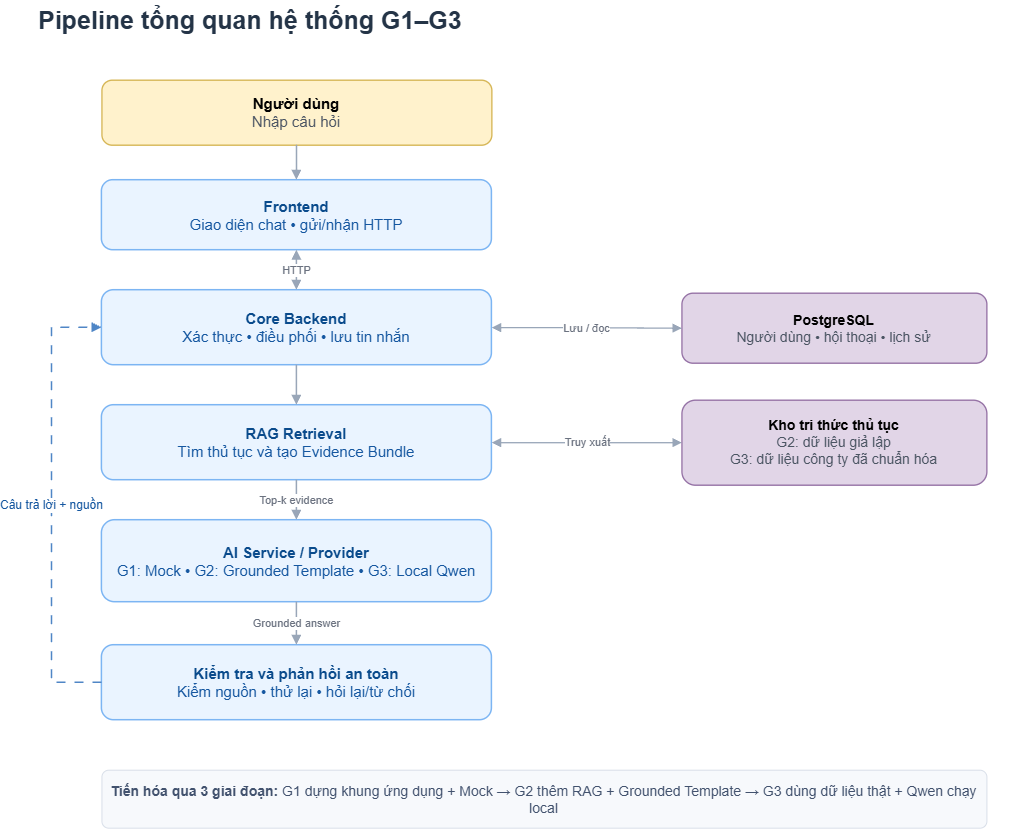
\includegraphics[width=0.76\textwidth]{system-pipeline.png}
    \caption{Pipeline tổng quan của hệ thống qua ba giai đoạn phát triển.}
    \label{fig:pipeline}
\end{figure}

Kiến trúc phần mềm được giữ ổn định trong khi thành phần dữ liệu và AI được nâng
cấp dần. Giai đoạn 1 dùng Mock AI để kiểm tra luồng ứng dụng. Giai đoạn 2 thêm RAG
và Grounded Template trên dữ liệu giả lập. Giai đoạn 3 thay dữ liệu giả bằng một
subset dữ liệu công ty và thay template bằng Qwen chạy local.

\subsection{Giai đoạn 1 -- Khung ứng dụng với Mock AI}

Mục tiêu của Giai đoạn 1 là xây dựng một luồng ứng dụng hoàn chỉnh trước khi tích
hợp dữ liệu hành chính và LLM thật. Hệ thống gồm giao diện React, Core Backend và
AI Service sử dụng FastAPI, PostgreSQL và Docker Compose.

Frontend chuyển câu hỏi tới Core Backend. Backend xác định người dùng, tạo hoặc
lấy cuộc hội thoại, lưu câu hỏi và gọi AI Service. Phản hồi mô phỏng được lưu vào
PostgreSQL rồi gửi lại giao diện. Giai đoạn này kiểm tra kết nối giữa các dịch vụ,
lưu lịch sử sau khi tải lại trang, tách dữ liệu giữa người dùng và tránh tạo tin
nhắn trùng lặp. Nhờ đó, lỗi giao diện, API và cơ sở dữ liệu được xử lý trước khi
bổ sung RAG.

\subsection{Giai đoạn 2 -- RAG trên dữ liệu giả lập}

Giai đoạn 2 xây dựng corpus giả lập gồm 3 thủ tục, 24 fragments và 33 câu hỏi đánh
giá. Trong đó, 23 câu thuộc DEV và 10 câu thuộc TEST. Corpus chỉ phục vụ kiểm thử
kỹ thuật và không được xem là hướng dẫn hành chính thực tế.

Dữ liệu gồm \textit{Source}, \textit{Procedure}, \textit{Fragment} và
\textit{Gold Question}. Trước khi ingest, pipeline kiểm tra schema, phiên bản, mã
định danh, quan hệ tham chiếu và mã băm nội dung.

Backend chuẩn hóa câu hỏi rồi kết hợp exact match, tìm từ khóa và BM25. Hệ thống
lấy tối đa 5 fragments phù hợp nhất; nếu nhiều thủ tục cùng khớp, hệ thống yêu
cầu làm rõ thay vì tự chọn. Các fragments được đóng gói thành
\textit{Evidence Bundle}. AI Service sử dụng Grounded Template offline, không
dùng Hosted API. Backend chỉ chấp nhận citation thuộc chính bundle của yêu cầu,
sau đó bổ sung thông tin nguồn, lưu kết quả và hiển thị trên web. Evidence rỗng
hoặc citation sai sẽ dẫn đến hỏi lại hoặc từ chối an toàn.

\subsection{Giai đoạn 3 -- Dữ liệu công ty và Qwen local}

Giai đoạn 3 đưa dữ liệu thực tế và Qwen vào kiến trúc đã được kiểm tra. Workbook
do công ty cung cấp chỉ được xử lý local, không đưa lên GitHub và không gửi tới
dịch vụ AI bên ngoài.

\subsubsection{Tiền xử lý dữ liệu}

Pipeline dữ liệu gồm các bước chính sau:

\begin{enumerate}
    \item Đọc workbook, nhận diện tiêu đề, ánh xạ cột và bỏ dòng trống. Pipeline
    dừng nếu cột có dữ liệu nhưng chưa có quy tắc xử lý.
    \item Loại email và metadata không cần thiết; quét số điện thoại, số định danh
    và chuỗi có dạng API key.
    \item Chuẩn hóa khoảng trắng và Unicode theo NFC; tạo ID và mã băm ổn định để
    kết quả có thể tái tạo.
    \item Ánh xạ các trường nghiệp vụ. Phí và thời gian chỉ được parse khi đủ chắc
    chắn; văn bản gốc được giữ để đối chiếu. Trường thiếu được ghi là
    \texttt{null} hoặc danh sách rỗng, không tự suy đoán.
    \item Cách ly bản ghi trùng tên nhưng xung đột; tạo fragments theo từng trường,
    rồi kiểm tra JSON Schema, tham chiếu, PII, phiên bản và mã băm trước khi phát
    hành corpus demo.
\end{enumerate}

\subsubsection{Corpus và phân chia dữ liệu}

Nhóm chọn subset gồm 10 thủ tục từ dữ liệu công ty, tạo thành 10 procedure và 49
fragments. Tổng cộng 40 câu hỏi được chia theo thủ tục thay vì chia ngẫu nhiên
theo từng câu. DEV gồm 8 thủ tục với 31 câu hỏi; TEST gồm 2 thủ tục với 9 câu hỏi.
TEST được khóa bằng mã băm và không dùng để sửa prompt, retrieval hoặc model.
Cách chia này hạn chế việc các câu gần giống của cùng một thủ tục xuất hiện ở cả
DEV và TEST.

\subsubsection{Sinh câu trả lời và kiểm tra an toàn}

Câu hỏi được định tuyến tới thủ tục phù hợp, sau đó exact match và BM25 chọn tối
đa 5 fragments để tạo \textit{Evidence Bundle}. AI Service sử dụng
Qwen3-1.7B Q8\_0 qua llama.cpp ở chế độ zero-shot, chưa fine-tune. Model chỉ nhận
câu hỏi và evidence cần thiết, không nhận toàn bộ workbook hoặc lịch sử người
dùng.

Qwen phải trả trạng thái, nội dung và danh sách fragment được trích dẫn theo một
output contract. Nếu output sai cấu trúc, hệ thống thử lại tối đa một lần. Nếu
vẫn sai nhưng evidence hợp lệ, hệ thống chuyển sang chế độ trích xuất an toàn từ
fragment đã duyệt. Câu thiếu tên thủ tục được yêu cầu làm rõ; câu không có bằng
chứng nhận trạng thái không đủ dữ liệu. Timeout, mất kết nối hoặc citation ngoài
bundle đều được xử lý theo hướng đóng an toàn.

\section{Results}

\subsection{Thiết lập thực nghiệm}

Hai thí nghiệm được chạy trên cùng máy local bằng Docker. Thí nghiệm 1 so sánh
Grounded Template và Qwen3-1.7B trên cùng 33 câu hỏi giả lập, cùng retrieval và
\textit{Evidence Bundle}. Thí nghiệm 2 đánh giá Qwen trên corpus công ty gồm 10
thủ tục và 49 fragments với Top-5 retrieval. Các chỉ số dưới đây đo routing,
retrieval, contract, citation và latency; chúng không thay thế đánh giá độ đúng
nghiệp vụ của chuyên gia.

\subsection{So sánh provider trên dữ liệu giả lập}

\begin{table}[t]
\centering
\small
\setlength{\tabcolsep}{4.5pt}
\begin{tabular}{@{}lrr@{}}
\toprule
\textbf{Chỉ số} & \textbf{Template} & \textbf{Qwen3-1.7B}\\
\midrule
Số câu hỏi & 33 & 33\\
Số lần gọi provider & 30 & 30\\
Độ chính xác trạng thái & 100\% & 100\%\\
Output hợp lệ & 100\% & 100\%\\
Citation binding hợp lệ & 100\% & 100\%\\
Gold citation recall & 60\% & 90\%\\
Unsafe answer rate & 0\% & 0\%\\
Extractive fallback & 0 & 0\\
Latency p50 (ms) & 2,525 & 625,485\\
Latency p95 (ms) & 14,425 & 708,000\\
\bottomrule
\end{tabular}
\caption{Kết quả Grounded Template và Qwen trên 33 câu hỏi giả lập.}
\label{tab:g2-comparison}
\end{table}

\tableref{tab:g2-comparison} cho thấy cả hai phương pháp đều tuân thủ trạng thái,
contract và citation. Template nhanh vì chỉ trích xuất theo quy tắc cố định. Qwen
có latency lớn hơn nhưng gold citation recall tăng từ 60\% lên 90\%, nghĩa là
model thường trích dẫn đúng fragment kỳ vọng hơn. Kết quả này không được diễn
giải thành độ chính xác pháp lý vì dữ liệu hoàn toàn giả lập và chưa có đánh giá
ngữ nghĩa của con người.

\subsection{Qwen trên dữ liệu công ty}

\begin{table}[t]
\centering
\small
\setlength{\tabcolsep}{5pt}
\begin{tabular}{@{}lrr@{}}
\toprule
\textbf{Chỉ số} & \textbf{DEV} & \textbf{TEST}\\
\midrule
Số câu hỏi & 31 & 9\\
Số lần gọi Qwen & 31 & 8\\
Routing accuracy & 100\% & 100\%\\
Retrieval Recall@5 & 80\% & 75\%\\
Độ chính xác trạng thái & 96,77\% & 88,89\%\\
Output hợp lệ & 100\% & 100\%\\
Citation binding hợp lệ & 100\% & 100\%\\
Lỗi HTTP & 0 & 0\\
Latency p50 (ms) & 668,271 & 666,458\\
Latency p95 (ms) & 1.160,768 & 1.257,099\\
Lời gọi AI bên ngoài & 0 & 0\\
\bottomrule
\end{tabular}
\caption{Kết quả Qwen trên DEV và TEST của corpus công ty.}
\label{tab:g3-results}
\end{table}

Trong TEST, một câu được guard xử lý mà không cần gọi model do không đủ điều kiện
sinh câu trả lời. \tableref{tab:g3-results} cho thấy toàn bộ câu hỏi được định
tuyến đúng thủ tục; output do Qwen tạo ra đều hợp lệ và citation đều thuộc
evidence đã cung cấp. Tuy nhiên, Recall@5 đạt 80\% trên DEV và 75\% trên TEST,
trong khi độ chính xác trạng thái TEST đạt 88,89\%. Sai số hiện tại vì vậy tập
trung nhiều hơn ở việc chọn fragment và quyết định trạng thái, thay vì lỗi kết
nối hoặc output contract.

\section{Future Work}

Các giai đoạn tiếp theo sẽ mở rộng từ 10 thủ tục sang corpus đã được phê duyệt và
cải thiện liên kết giữa ý định câu hỏi với loại bằng chứng. Dense retrieval và
reranker chỉ được bổ sung khi phân tích lỗi chứng minh BM25 chưa đáp ứng. Hệ thống
cũng cần hiểu câu hỏi nối tiếp, ghi nhớ thủ tục đang trao đổi và quản lý ngữ cảnh
dài hơn. Fine-tune hoặc QLoRA chỉ được xem xét khi có dữ liệu huấn luyện đã duyệt
và lỗi diễn giải lặp lại được xác định rõ.

Trước khi triển khai thực tế, cần xây dựng TEST mới có đánh giá nghiệp vụ, đồng
thời bổ sung xác thực, phân quyền, giám sát, xử lý đồng thời và quy trình cập nhật
dữ liệu. Câu trả lời phải hiển thị phiên bản nguồn, thời điểm hiệu lực và cảnh báo
rằng hệ thống không thay thế cơ quan có thẩm quyền.

\section{Conclusion}

Dự án đã phát triển từ khung ứng dụng dùng Mock AI, sang RAG trên dữ liệu giả lập,
rồi tới hệ thống dùng 10 thủ tục công ty, 49 fragments và Qwen3-1.7B local. Kết
quả cho thấy pipeline Docker hoạt động xuyên suốt; output và citation tuân thủ
contract mà không gửi dữ liệu công ty tới Hosted API. Retrieval và quyết định
trạng thái vẫn cần cải thiện. Vì vậy, đây là nền tảng demo nội bộ hoàn chỉnh về
luồng kỹ thuật, chưa phải sản phẩm sẵn sàng triển khai thực tế.

\section{Video Demo}

\noindent\href{https://drive.google.com/drive/folders/1iMOLAEUCQz8EJg_uvCxlsPn2mnr5dAB8?usp=sharing}
{\textbf{Video demo hệ thống LLM tư vấn pháp lý cơ bản}}

\end{document}
